%!TEX root = main.tex

\begin{figure*}[htbp]
	\centering
	\newcommand\myheight{0.131}
	\subfloat[] {
		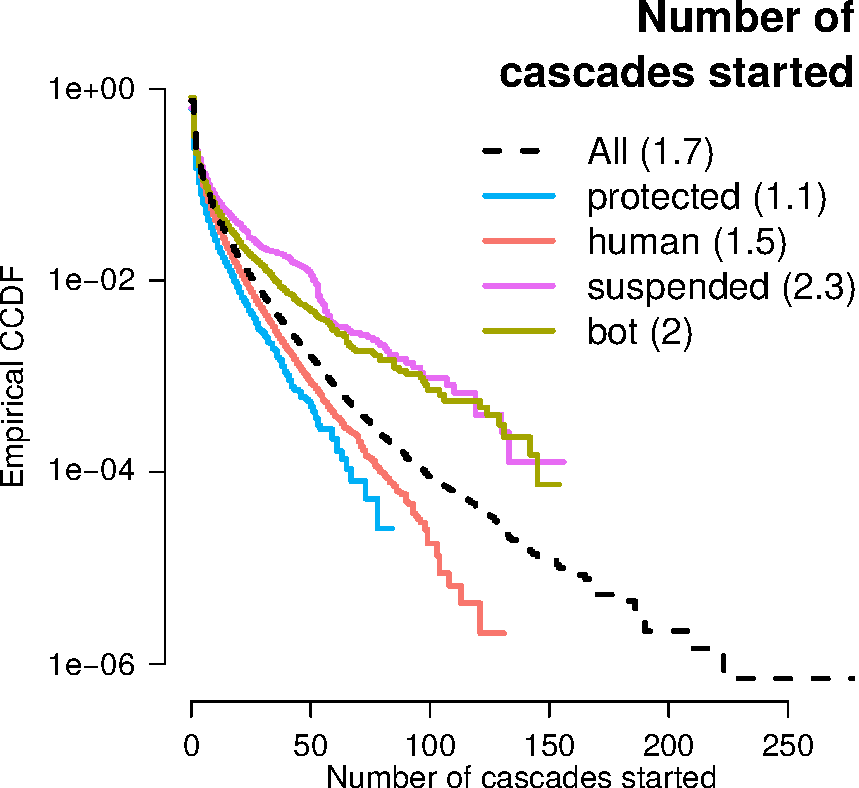
\includegraphics[height=\myheight\textheight]{bot-a-number-of-diffusions}
		\label{subfig:no-cascades}
	}
	\subfloat[] {
		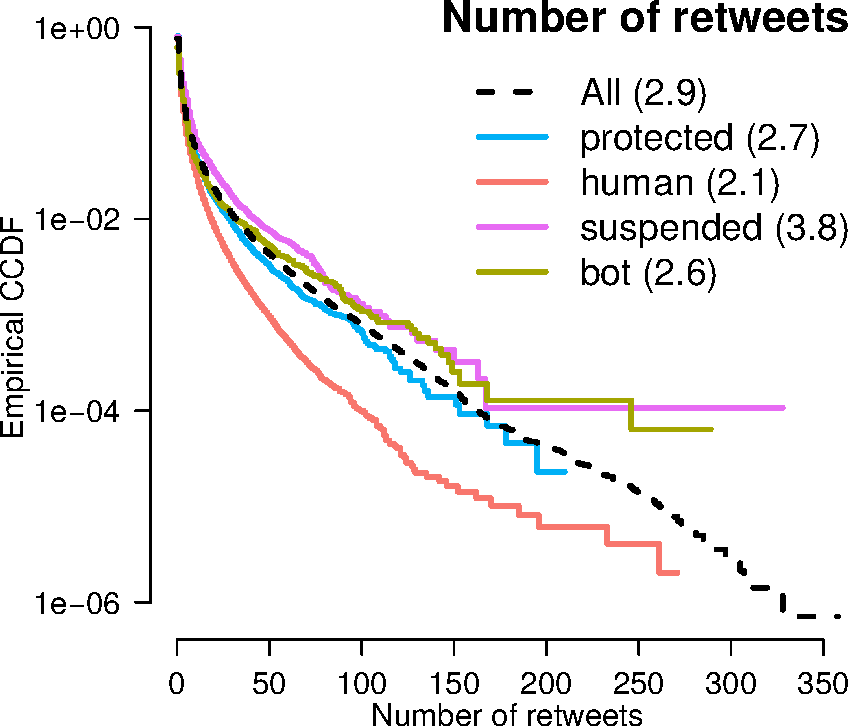
\includegraphics[height=\myheight\textheight]{bot-b-number-of-retweets}
		\label{subfig:no-retweets}
	}
	\subfloat[] {
		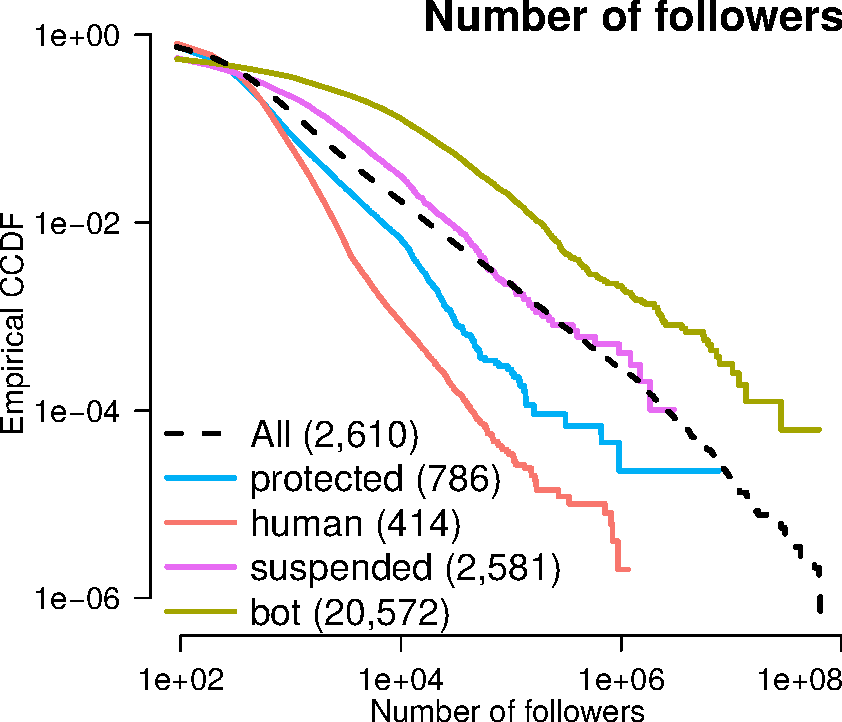
\includegraphics[height=\myheight\textheight]{bot-c-followers-count-CCDF}
		\label{subfig:numfolowers-CCDF}
	}
	\subfloat[] {
		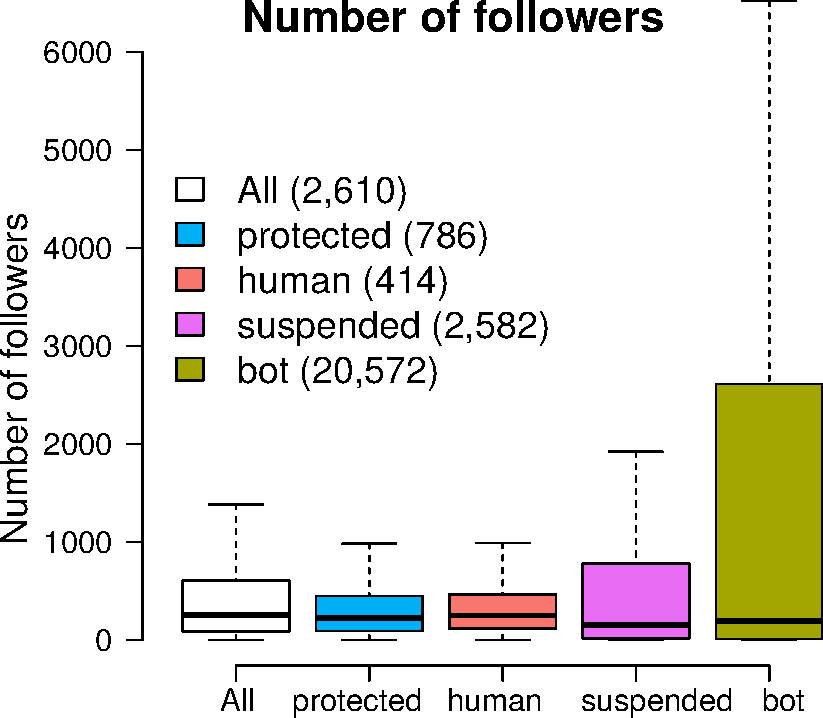
\includegraphics[height=\myheight\textheight]{bot-d-followers-count-boxplot}
		\label{subfig:numfolowers-boxplot}
	}
	\subfloat[] {
		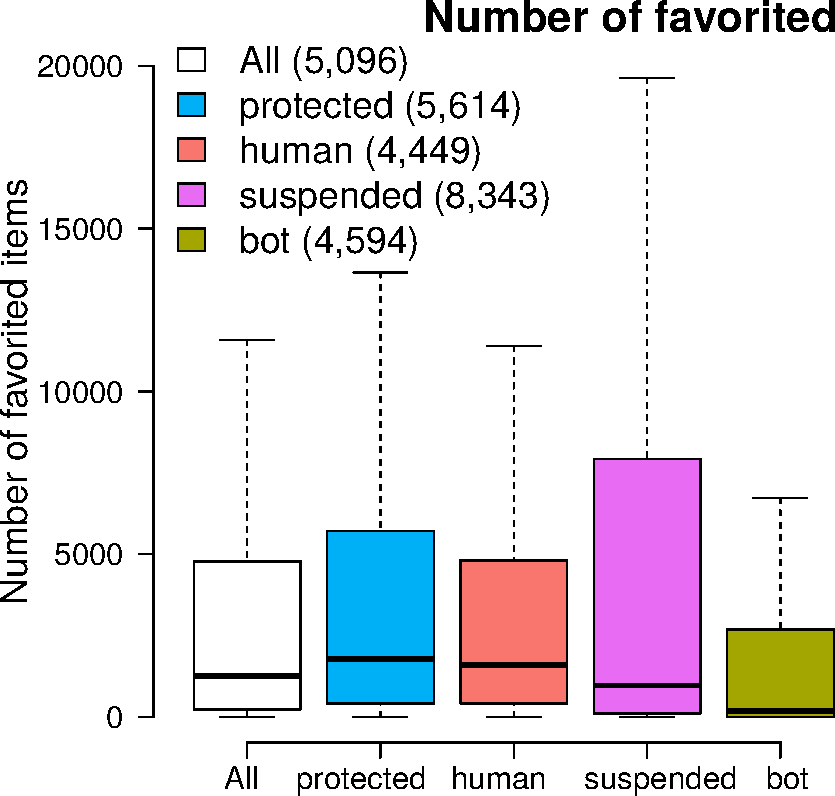
\includegraphics[height=\myheight\textheight]{bot-e-favorites-count}
		\label{subfig:numfavorited}
	}
	\caption{ 
		Profiling behavior of the \Protected, \Human, \Suspended and \Bot populations in the \debate dataset.
		The numbers in parentheses in the legend are mean values.
		\textbf{(a)} CCDF of the number of Twitter diffusion cascades started.
		\textbf{(b)} CCDF of the number of retweets. 
		\textbf{(c)(d)} CCDF (c) and boxplots (d) of the number of followers. 
		\textbf{(e)} Number of items favorited.
	}
	\label{fig:bot-profiling}
%	\captionmoveup
\end{figure*}